\documentclass[compress,xcolor=table]{beamer}

\usepackage{lmodern}
\usepackage[utf8]{inputenc}

\mode<presentation>
{
	\usetheme{Madrid}      % or try Darmstadt, Madrid, Warsaw, ...
	\usecolortheme{seahorse} % or try albatross, beaver, crane, ...
	\usefonttheme{serif}  % or try serif, structurebold, ...
	\setbeamertemplate{navigation symbols}{}
	\setbeamertemplate{caption}[numbered]
} 

\makeatletter
\setbeamertemplate{headline}{%
	\begin{beamercolorbox}[ht=2.25ex,dp=3.75ex]{section in head/foot}
		\insertnavigation{\paperwidth}
	\end{beamercolorbox}%
}%
\makeatother

\makeatletter
\newenvironment{withoutheadline}{
	\setbeamertemplate{headline}[default]
	\def\beamer@entrycode{\vspace*{-\headheight}}
}{}
\makeatother

\usepackage[english]{babel}
\usepackage[utf8]{inputenc}
\usepackage{xcolor}
\usepackage{listings}
\usepackage{textpos}
\newcommand\citem[1]{\item[{[#1]}] }

\lstset
{
	language=[LaTeX]TeX,
	breaklines=true,
	basicstyle=\tt\scriptsize,
	%commentstyle=\color{green}
	keywordstyle=\color{red},
	%stringstyle=\color{black}
	identifierstyle=\color{orange},
}

\newcommand{\backupbegin}{
	\newcounter{finalframe}
	\setcounter{finalframe}{\value{framenumber}}
}
\newcommand{\backupend}{
	\setcounter{framenumber}{\value{finalframe}}
}

\newenvironment<>{varblock}[2][.9\textwidth]{%
	\setlength{\textwidth}{#1}
	\begin{actionenv}#3%
		\def\insertblocktitle{#2}%
		\par%
		\usebeamertemplate{block begin}}
	{\par%
		\usebeamertemplate{block end}%
\end{actionenv}}

%\usepackage{outlines}
\setbeamercolor{itemize item}{fg=red,bg=white}

\usepackage{multirow}
\usepackage{caption}
\usepackage{subcaption}

\usepackage{animate}

\newcommand\pro{\item[$+$]}
\newcommand\con{\item[$-$]}

\usepackage[edges]{forest}
\usetikzlibrary{shadows,arrows.meta}
\usepackage{tcolorbox}
%Defining the styles used in trees
%Note that the fill colour is not defined here.
\tikzset{parent/.style={align=center,text width=2cm,rounded corners=2pt},
	child/.style={align=center,text width=7.5cm,rounded corners=6pt},
	grandchild/.style={align=left, text width=13cm}
}

\newcommand\blfootnote[1]{%
	\begingroup
	\renewcommand\thefootnote{}\footnote{#1}%
	\addtocounter{footnote}{-1}%
	\endgroup
}

%%% TITLE
\title[Globecom 2021]{On the Performance of Blockchain-enabled RAN-as-a-service in Beyond 5G Networks}
\author[Wilhelmi, F., and Giupponi, L.]{
\includegraphics[width=\textwidth,height=0.13\textheight,keepaspectratio]{img/cttc}\\~\\ \textbf{Francesc Wilhelmi} and Lorenza Giupponi}
\institute[]{Globecom 2021}
\date[7-11 December 2021]{7-11 December 2021}

\AtBeginSection[]
{
	\begin{frame}<beamer>
	\frametitle{Outline}
	\tableofcontents[currentsection,currentsubsection]
\end{frame}
}

\begin{document}

\begin{withoutheadline}
	\begin{frame}
		\titlepage
	\end{frame}
\end{withoutheadline}

\begin{frame}{Table of contents} % and our simple frame
	\tableofcontents
\end{frame}

%%%%%%%%%%%%%%
%%% Motivation
%%%%%%%%%%%%%%
\section[Introduction]{Introduction and Related Work}

\subsection{}
\begin{frame}{Towards Blockchain-enabled Communications}
	\begin{block}{RAN sharing in 5G/6G}
			\begin{itemize}
				\item Need for fostering economic sustainability
				\item Push towards decentralized solutions
				\item Exchanging resources among untrusted parties
			\end{itemize}
		\end{block}	
	\pause
		\begin{exampleblock}{Blockchain}
			\begin{itemize}
				\item Open telecom market without centralized management
				\item Immutability, transparency, and security
				\item Automation of definition and enforcement of SLAs
			\end{itemize}
		\end{exampleblock}	
	\pause
		\begin{center}
	\begin{minipage}{10cm}
		\begin{alertblock}{}
			\centering
			\scriptsize \textbf{Need for understanding the impact of BC over wireless networks}
		\end{alertblock}
	\end{minipage}
\end{center}
\end{frame}

\subsection{}
\begin{frame}{Main contributions}

\begin{columns}
		\begin{column}{5cm}
		\begin{figure}
			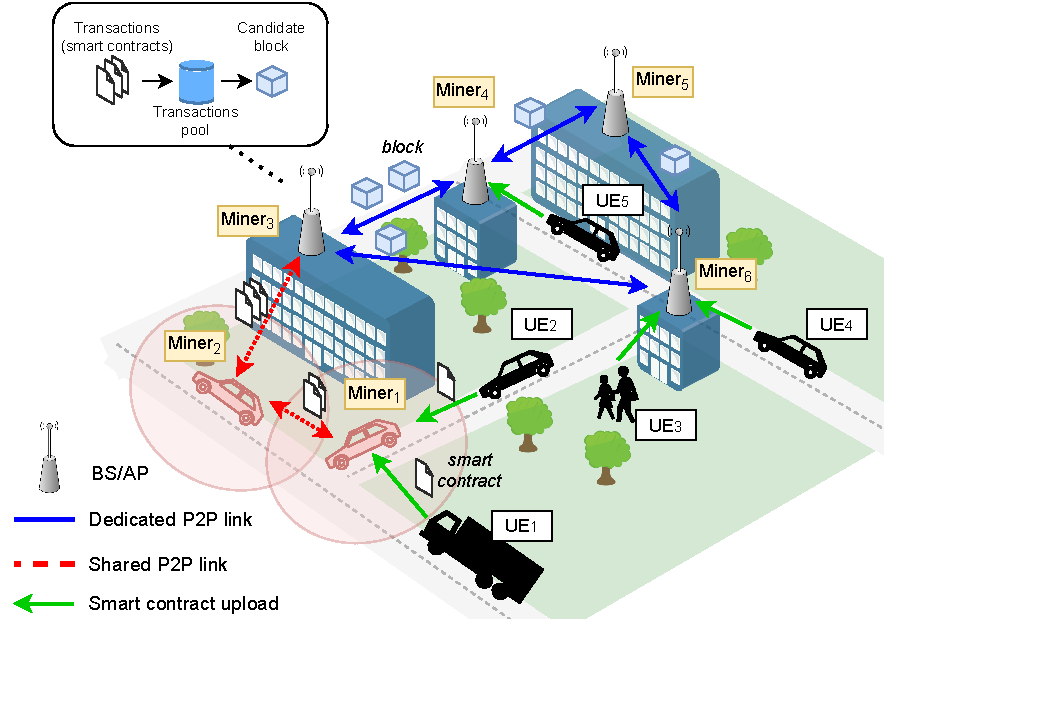
\includegraphics[width=\textwidth,keepaspectratio]{img/blockchain_ecosystem}\caption{\scriptsize Envisioned BC-enabled RAN ecosystem}
		\end{figure}
	\end{column}
	\begin{column}{6.7cm}
		\begin{enumerate}
			\item We foresee a BC-enabled RANaaS scenario for sharing resources
			\item We study the performance of BC (wired vs wireless)
		\end{enumerate}
	\end{column}
\end{columns}
	\vspace{-0.5cm}
	%\pause
%	\begin{minipage}{12cm}
%		\begin{alertblock}{}
%			\scriptsize All the source code used in this project is of open access and completely available:
%			\begin{itemize}
%				\item BC batch-service queue simulator: \url{https://github.com/fwilhelmi/batch_service_queue_simulator}
%				\item Model implementation: \url{https://bitbucket.org/francesc_wilhelmi/model_blockchain_delay}		
%		\end{itemize}
%		\end{alertblock}
%	\end{minipage}
\end{frame}

\subsection{}
\begin{frame}{Important references}
	\begin{exampleblock}{Blockchain \& RAN}
		\begin{itemize}
			\item Ecosystem: \cite{maksymyuk2020blockchain, xu2020blockchain}
			\item Architectural integration: \cite{xu2021ran}
		\end{itemize}		
	\end{exampleblock}
\pause
	\begin{block}{Slice broker}			
		\begin{itemize}
			\item Enabler for dynamic resource leasing %5G Network Slice Broker concept aims to enable mobile virtual network operators, over-the-top providers, and industry vertical market players to request and lease resources from infrastructure providers dynamically according to needs
			\item Previous work: \cite{backman2017blockchain, nour2019blockchain}
		\end{itemize}			
	\end{block}
\pause
\begin{alertblock}{Our contribution}			
	\begin{itemize}
		\item Broader view on RAN ecosystem (operators + UEs)
		\item Hybrid BC system (\cite{fan2020hybrid})
	\end{itemize}			
\end{alertblock}

\end{frame}


%%%%%%%%%%%%%%
%%% BC RAN
%%%%%%%%%%%%%%
\section{BC-enabled dynamic RAN sharing}

\subsection{}
\begin{frame}{Basics on Blockchain technology}
\begin{figure}
	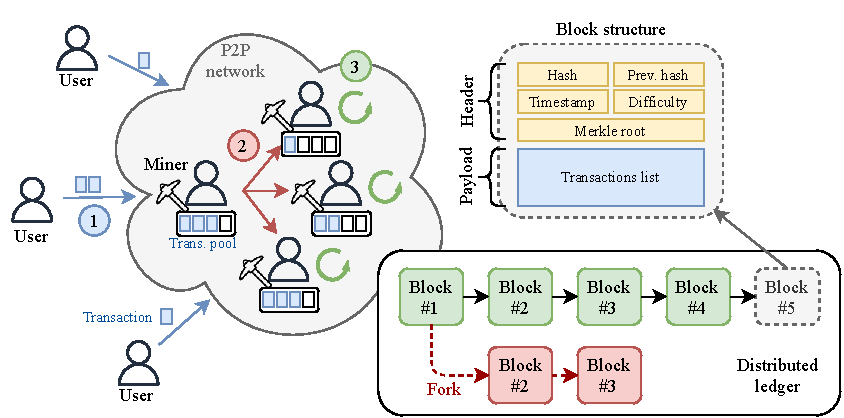
\includegraphics[width=\textwidth,keepaspectratio]{img/blockchain}\caption{\scriptsize Blockchain (BC) overview}
\end{figure}
\end{frame}

\subsection{}
\begin{frame}{RAN-as-a-Service (RANaaS) ecosystem}
\begin{columns}
	\begin{column}{5.5cm}
		\begin{block}{UEs}
			\begin{enumerate}
				\item Not tied to a single operator
				\item On-demand service requests
				\item Subscribe based on e.g., offered price, QoS, reputation
			\end{enumerate}		
		\end{block}		
	\end{column}
	\pause
	\begin{column}{5.5cm}	
		\begin{exampleblock}{Operators, providers}
			\begin{enumerate}
				\item Exchange radio \& infrastructure resources
				\item Based on dynamic demand
				\item Set prices based on expenses, e.g., equipment, site build-out, licenses
			\end{enumerate}		
		\end{exampleblock}		
	\end{column}		
\end{columns}
%\begin{center}
%	\begin{minipage}{9cm}
%		\begin{alertblock}{}
%			\centering
%			Enabled by reverse-auction mechanisms
%		\end{alertblock}
%	\end{minipage}		
%\end{center}

\end{frame}

\subsection{}
\begin{frame}{Blockchain for RA automation and auditability}
\begin{columns}
	\begin{column}{5.5cm}
		\begin{block}{Blockchain types}
			\begin{enumerate}
				\item Service blockchain (public)
				\item RAN blockchain (private)
			\end{enumerate}		
		\end{block}
		\pause
		\begin{exampleblock}{Functionalities}
			\begin{enumerate}
				\item Record transactions
				\item Enable auctions
				\item Payment by enforcing SCs
			\end{enumerate}		
		\end{exampleblock}
	\end{column}
	\pause
	\begin{column}{5.8cm}	
		\begin{figure}
			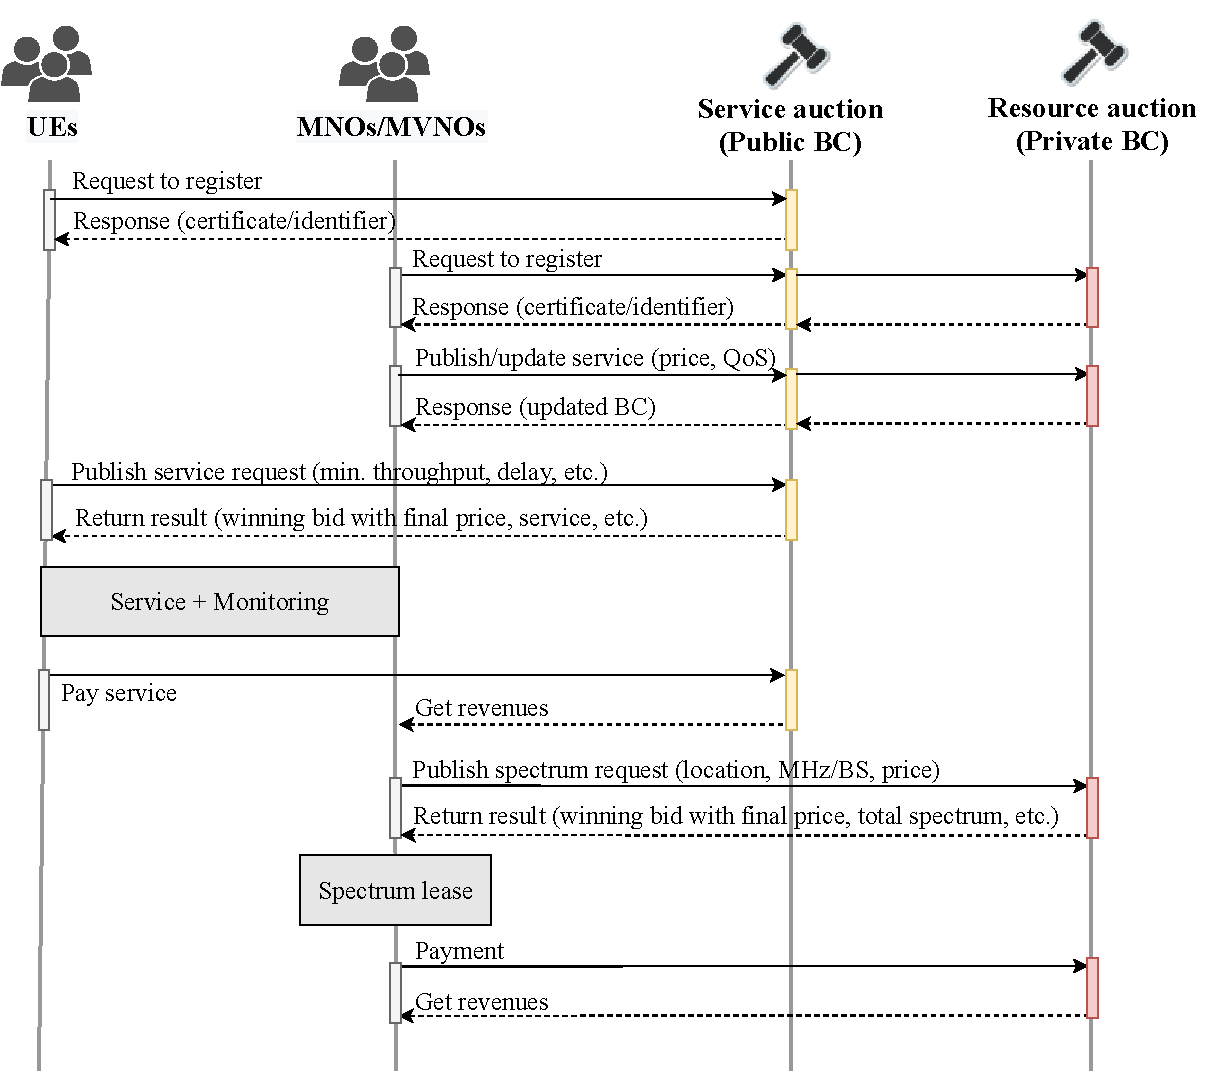
\includegraphics[width=\textwidth,keepaspectratio]{img/ra_options}\caption{\scriptsize BC-enabled RA procedures}
		\end{figure}
	\end{column}		
\end{columns}
\end{frame}

%%%%%%%%%%%%%%
%%% SYSTEM MODEL
%%%%%%%%%%%%%%
\section{System model}

\subsection{}
\begin{frame}{Blockchain transaction confirmation delay}

\begin{block}{Steps}
	\begin{enumerate}
		\item Users submit transactions to peer nodes ($T_\text{up}$) %The incurred delay depends on the utilized communications technology (e.g., IEEE 802.11, 5G NR). 
		%
		\item Collect transactions to fill a candidate block ($T_\text{queue}$)\footnote{More details in~\cite{wilhelmi2021discrete}}
		%
		\item Miners run consensus ($T_\text{mine}$)
		\item The winning miner propagates the mined block ($T_\text{prop}$)
	\end{enumerate}
\end{block}

\begin{equation}
T_\text{c} = T_\text{up} + \frac{(T_\text{queue} + T_\text{mine} + T_\text{prop})}{1-p_\text{fork}} \nonumber
\end{equation}

\end{frame}

\subsection{}
\begin{frame}{Other performance metrics}

\textbf{UE performance:}
\begin{equation}
C_n = b_n \log_2(1 + \text{SINR}_n) \nonumber
\end{equation}

\textbf{UE service acceptance:}
\begin{equation}
A_n(t) = 1-\exp{(-K \cdot b_{n}^{\psi} \cdot p^\xi)} \nonumber
\label{eq:acceptance}
\end{equation}


\end{frame}


%%%%%%%%%%%%%%
%%% PERF. EVALUATION
%%%%%%%%%%%%%%
\section{Numerical results}

\subsection{}
\begin{frame}{Simulation scenario}
\begin{columns}
	\begin{column}{6.5cm}
		\begin{block}{Scenario}
			\begin{itemize}
				\item Random cellular  deployment
					\begin{itemize}
						\item 19 BSs acting as miners
					\end{itemize}
				\item BC links
				\begin{itemize}
					\item Public (UEs): IEEE 802.11ax
					\item Private (operators): 5G NR X2/Xn
				\end{itemize}
				\item Simulation-driven analysis
			\end{itemize}
		\end{block}
	\end{column}
	\begin{column}{4.5cm}
		\begin{figure}
			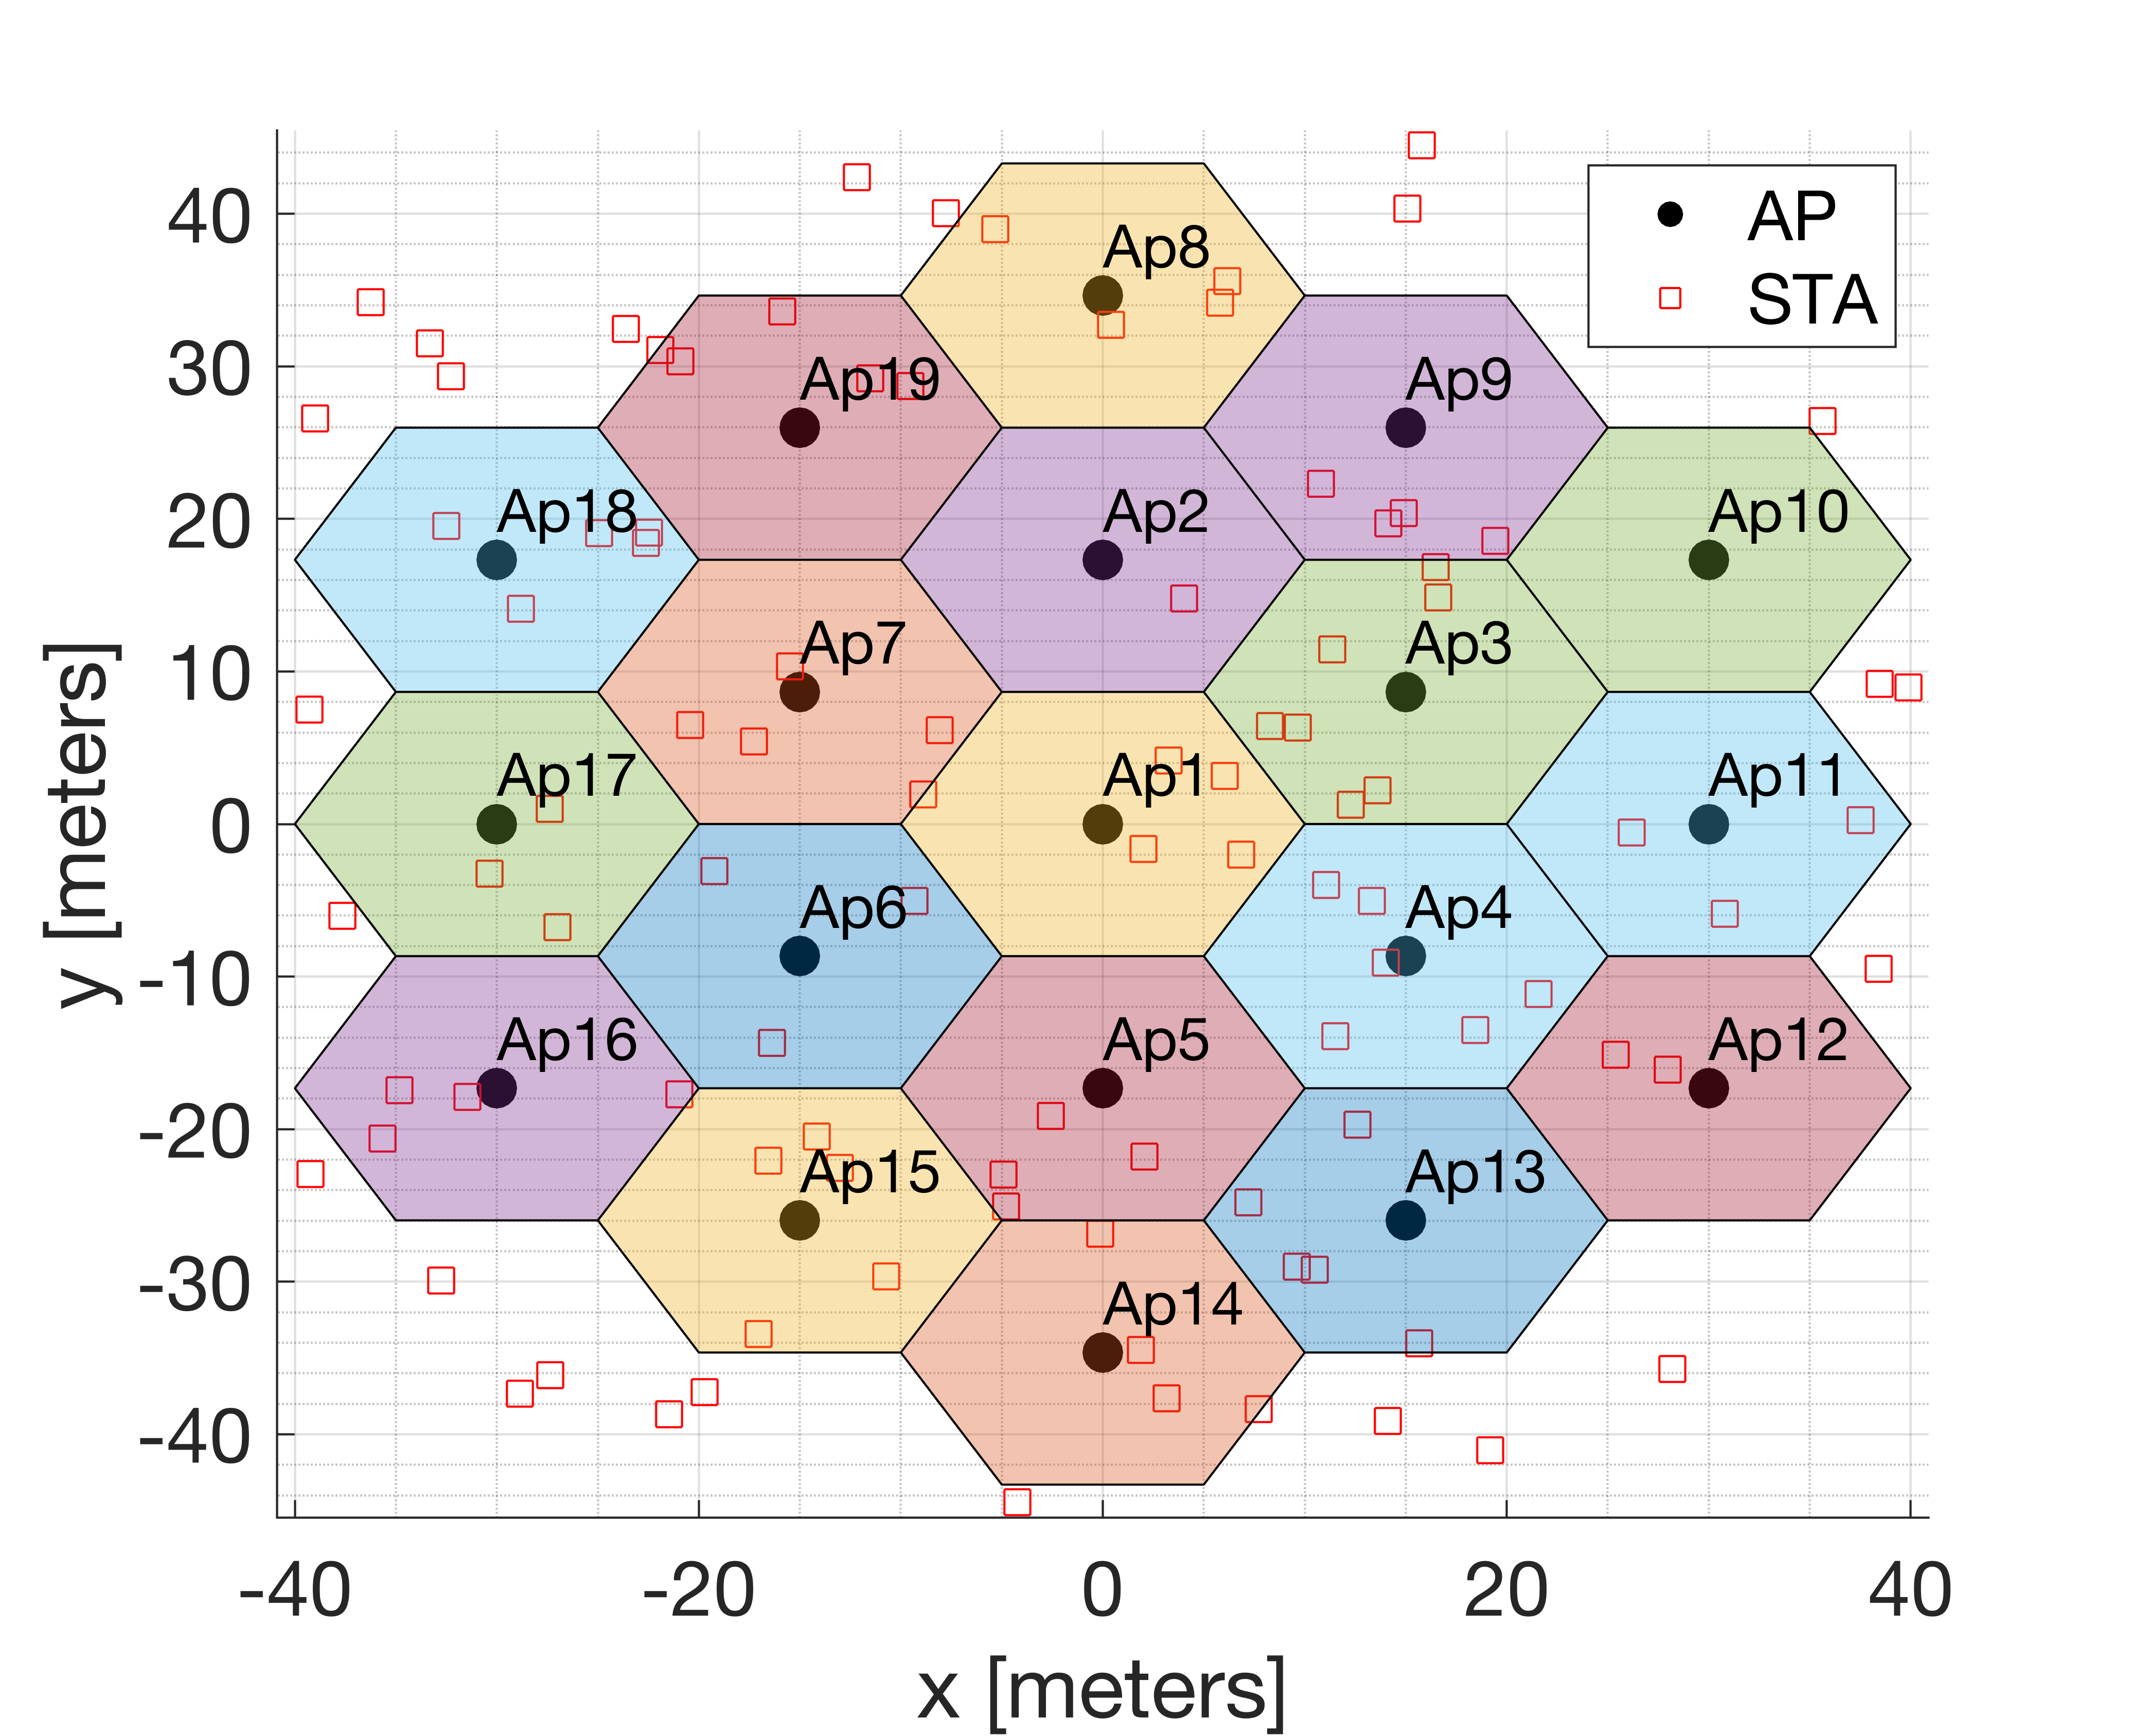
\includegraphics[width=\textwidth,keepaspectratio]{img/random_deployment}\caption{\scriptsize Simulation scenario}
		\end{figure}
	\end{column}
\end{columns}

\scriptsize \textbf{Note:} The code used in this paper is of open access, available at \url{https://github.com/fwilhelmi/blockchain_ran_sharing_simulator}

\end{frame}


\subsection{}
\begin{frame}{Analysis of the confirmation delay}
\begin{columns}
	\begin{column}{5cm}
		\begin{itemize}
			\item Arrivals ($\lambda$)
			\item Block size ($S^B$)
			\item Max. waiting time ($T_w$)
			\item 802.11ax or X2/Xn
		\end{itemize}
	\end{column}
	\begin{column}{6cm}
		\begin{figure}
			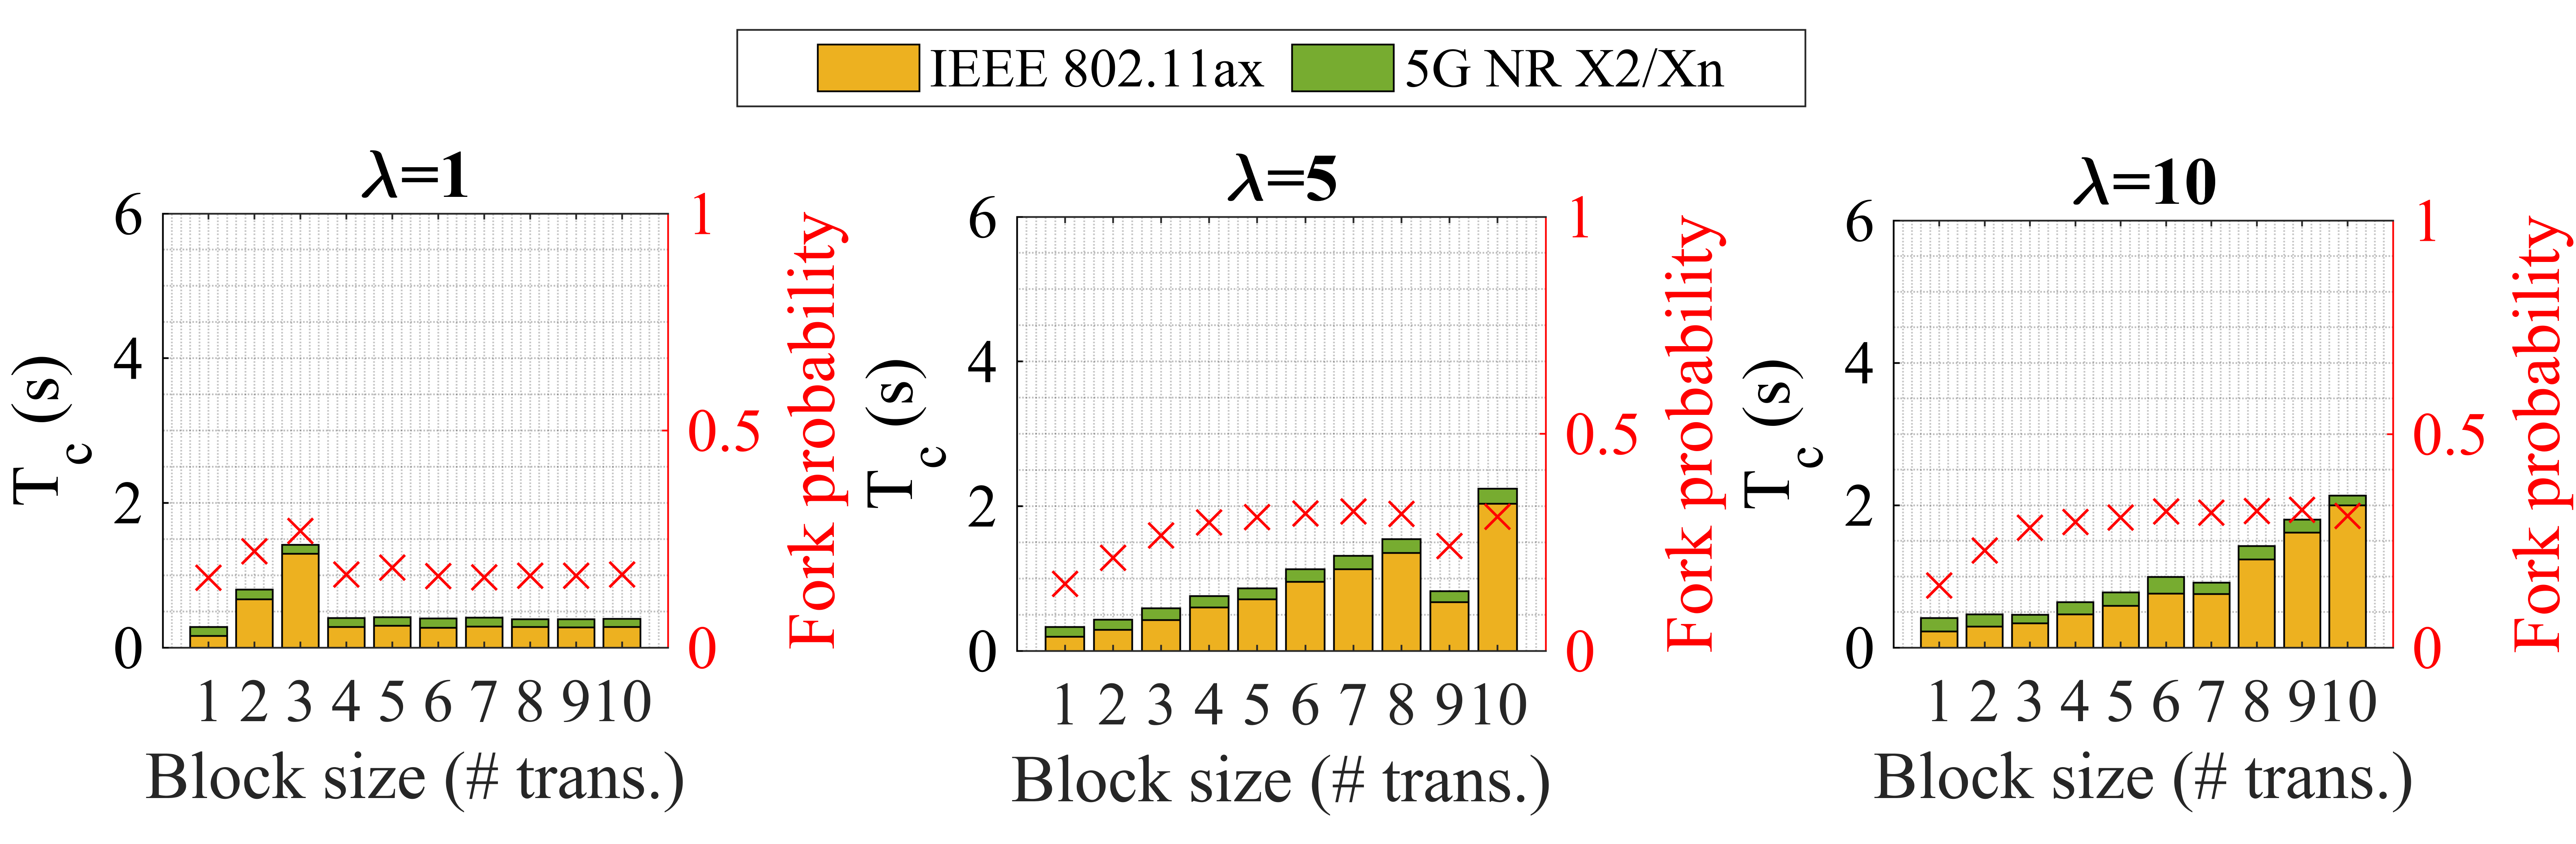
\includegraphics[width=\textwidth,keepaspectratio]{img/delays_with_forks_timer01}\caption{\scriptsize $T_\text{wait}=0.1$s}
		\end{figure}
		\vspace{-.8cm}
		\begin{figure}
			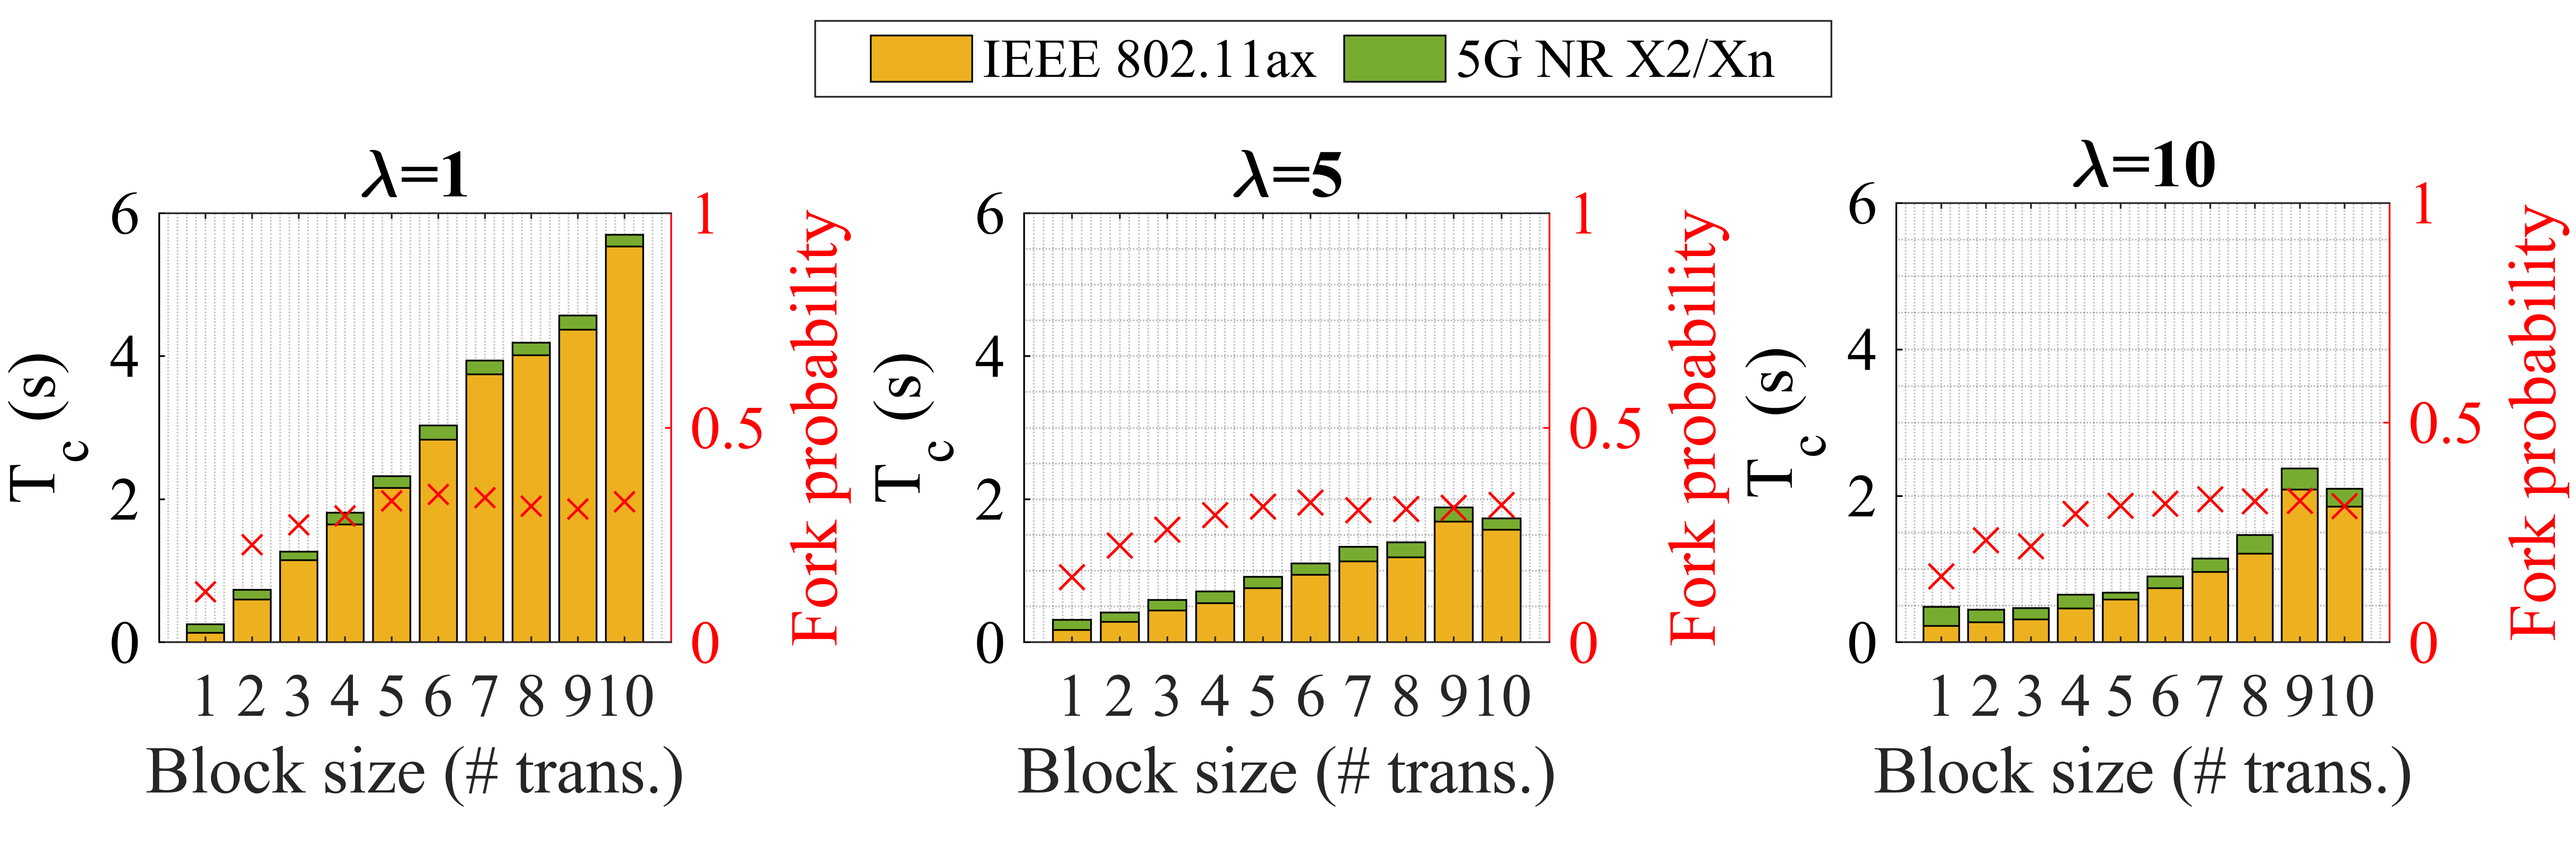
\includegraphics[width=\textwidth,keepaspectratio]{img/delays_with_forks_timer5}\caption{\scriptsize $T_\text{wait}=5$s}
		\end{figure}
	\end{column}
\end{columns}
\end{frame}

\subsection{}
\begin{frame}{UE performance}
\begin{columns}
	\begin{column}{5cm}
		\begin{itemize}
			\item RAN sharing type:
			\begin{enumerate}
				\item \textbf{Static:} no exchange
				\item \textbf{Dynamic:} BC-based auction
			\end{enumerate}
			\item User traffic profiles: 
			\begin{enumerate}
				\item Low
				\item Average
				\item High
			\end{enumerate}
			\item $M$ sharing operators
	\end{itemize}
	\end{column}
	\begin{column}{6cm}
		\begin{figure}
			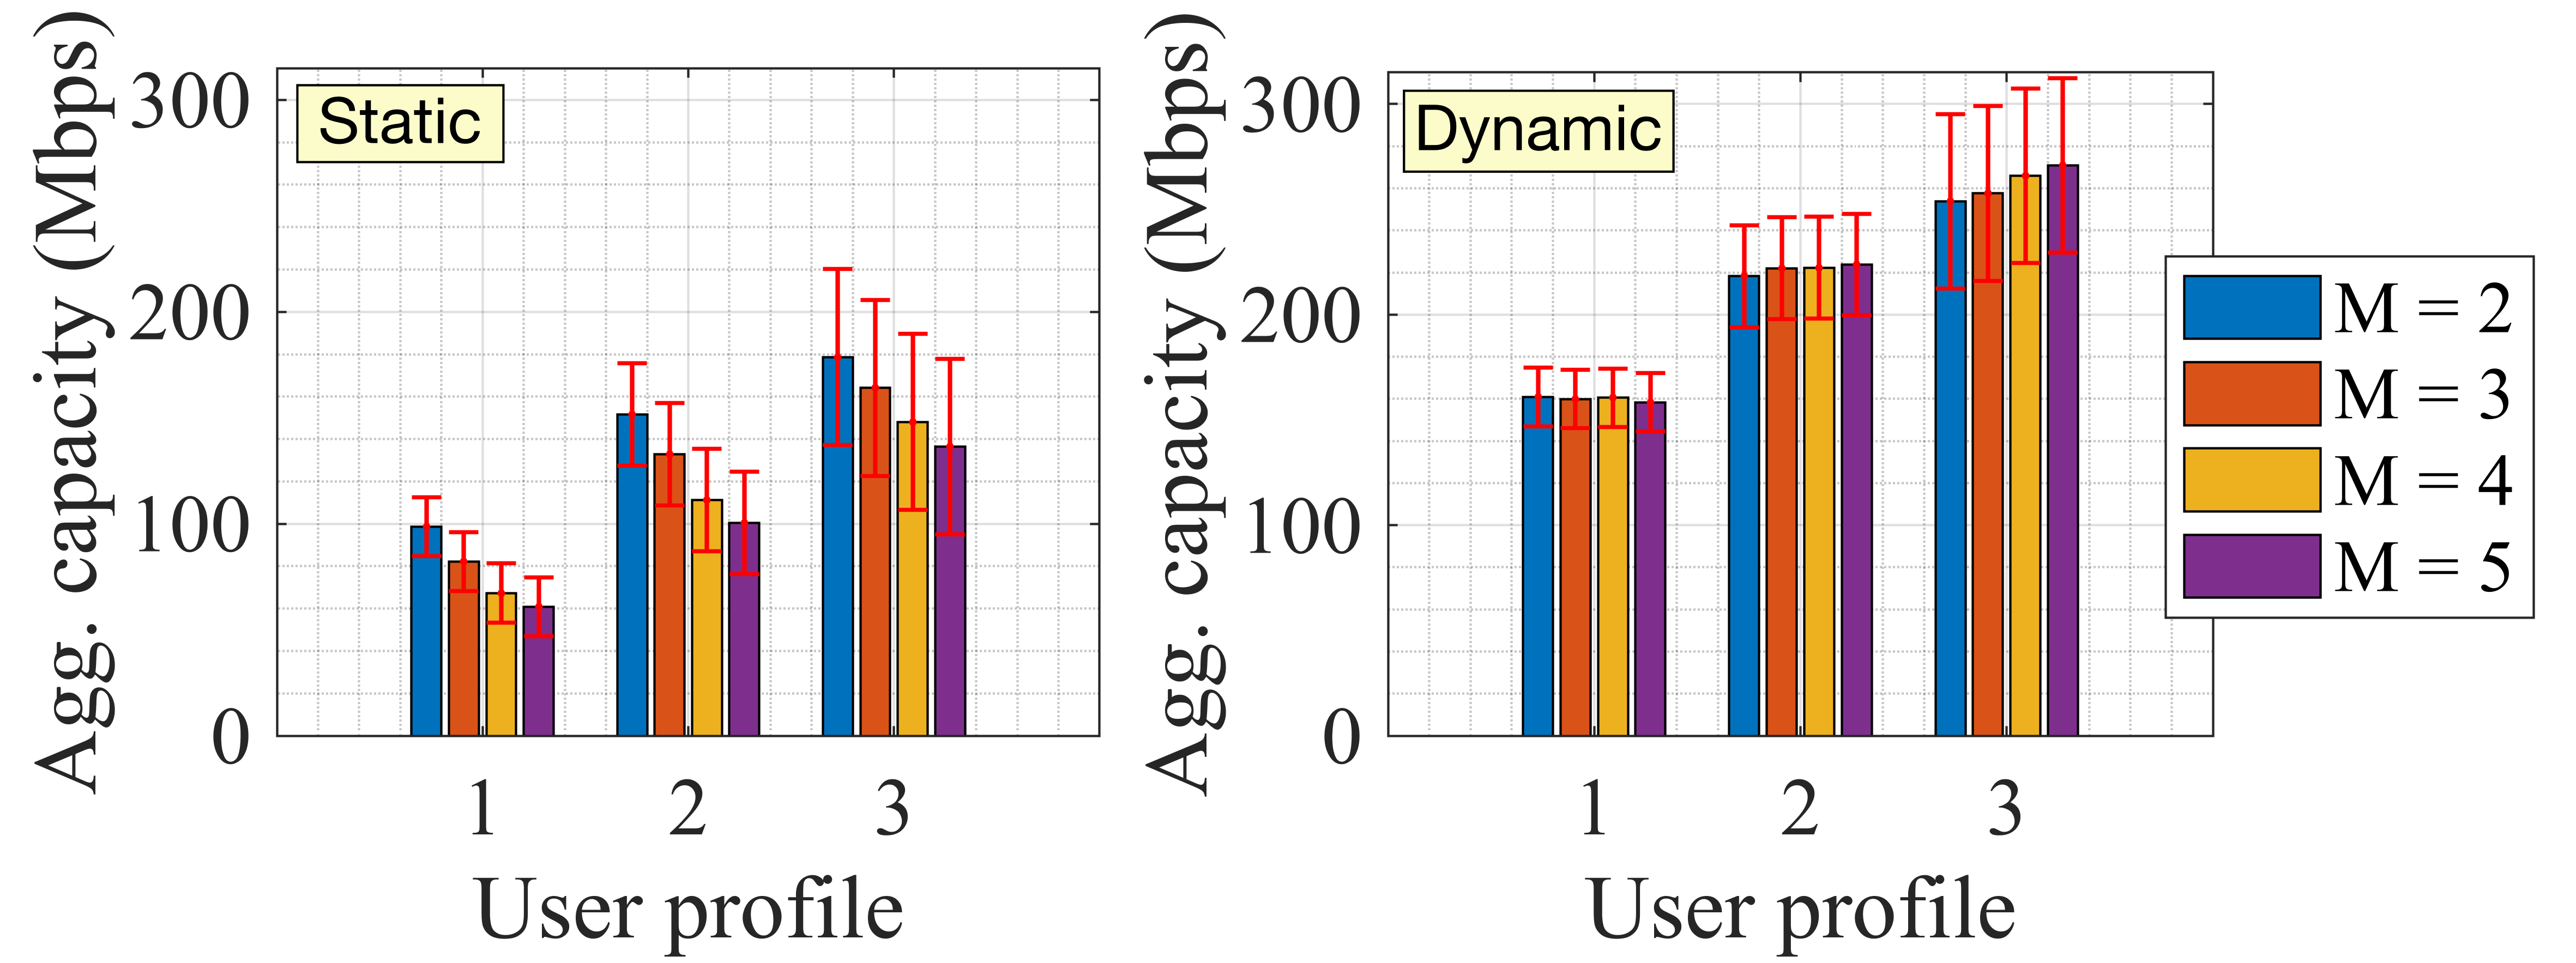
\includegraphics[width=\textwidth,keepaspectratio]{img/capacity_random}\caption{\scriptsize Capacity}
		\end{figure}
		\vspace{-.8cm}
		\begin{figure}
			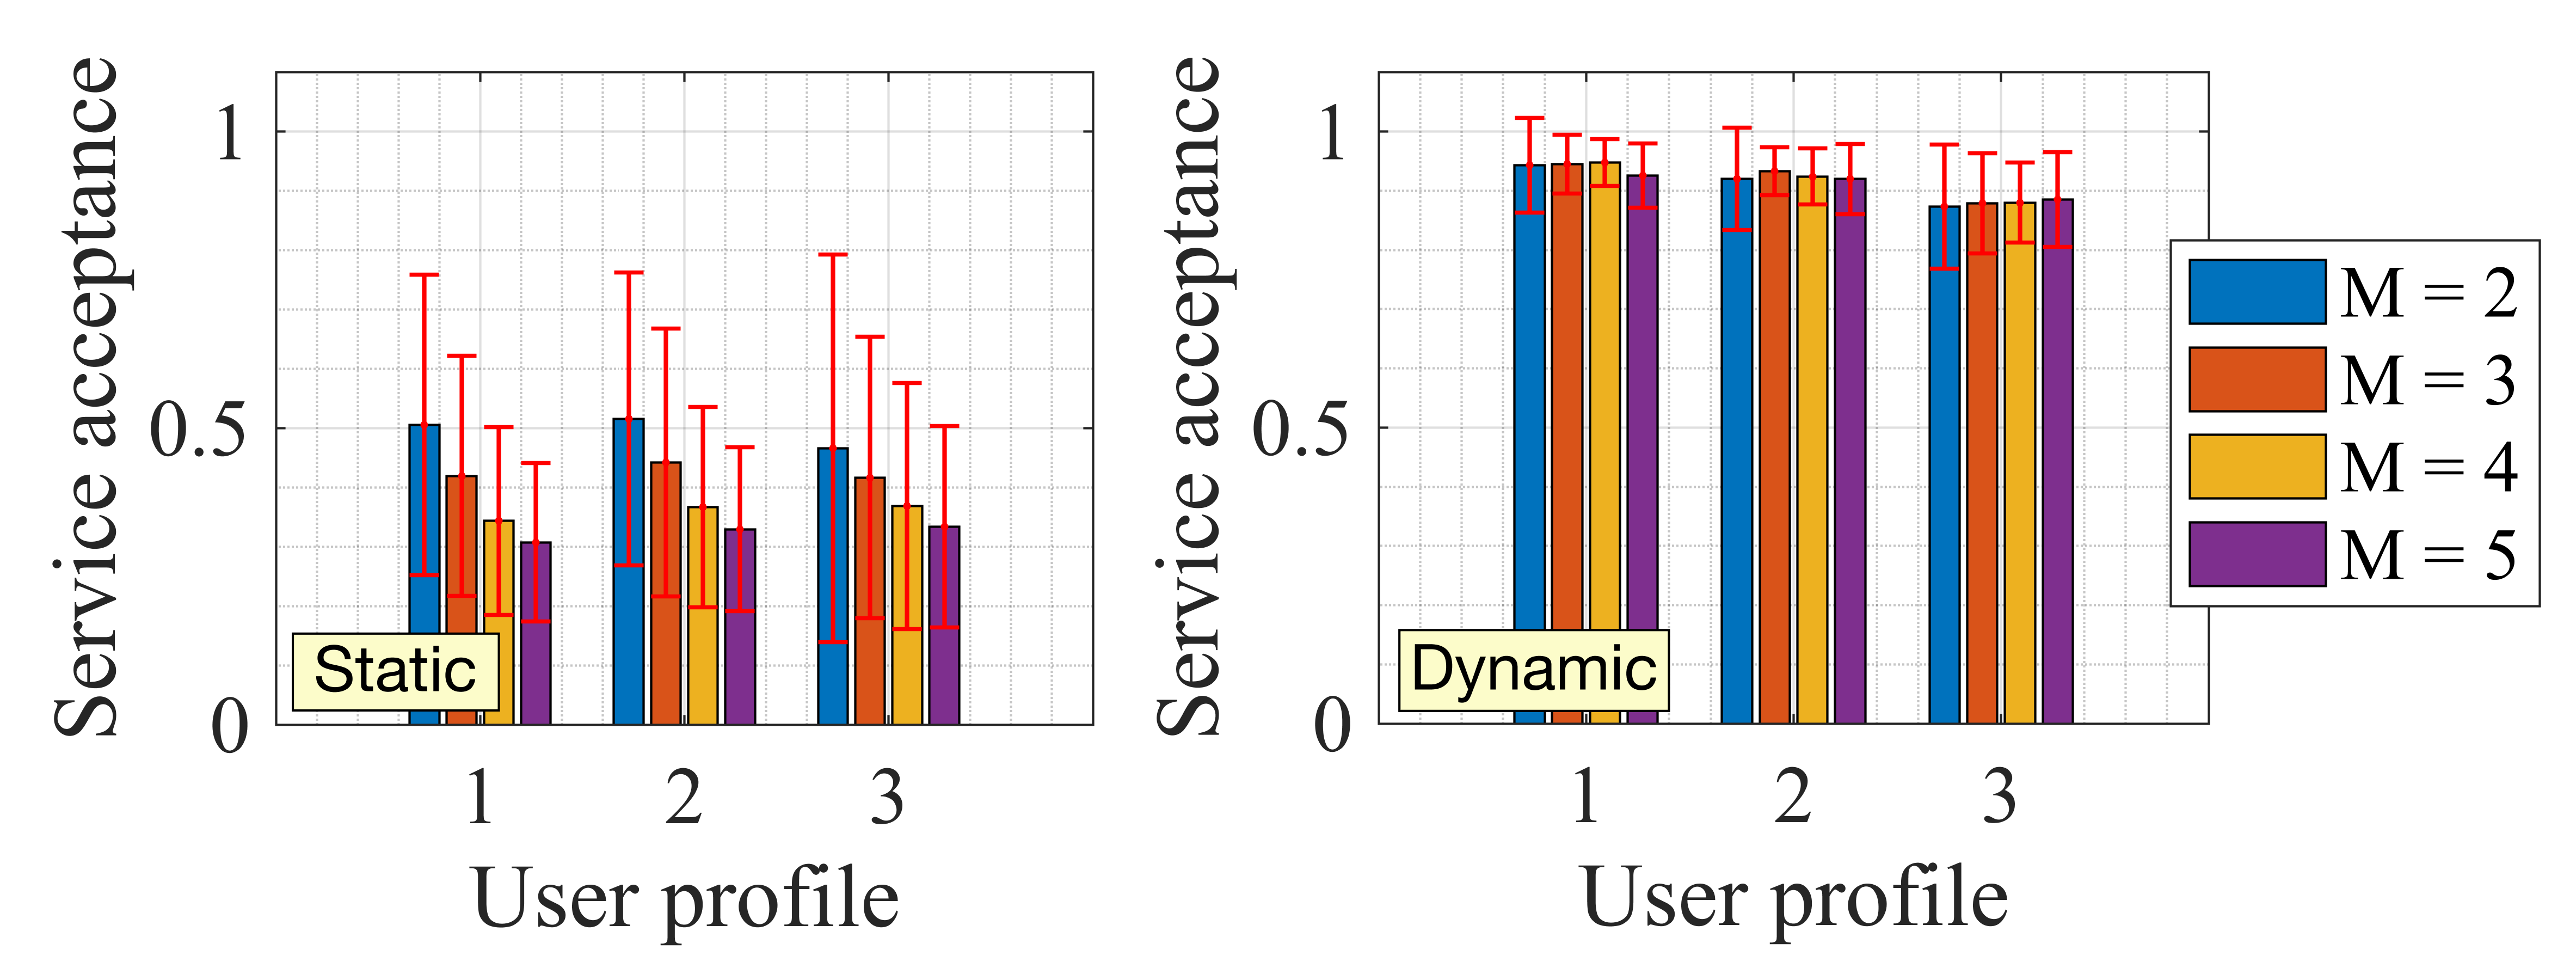
\includegraphics[width=\textwidth,keepaspectratio]{img/service_acceptance_random}\caption{\scriptsize Service acceptance}
		\end{figure}
	\end{column}
\end{columns}
\end{frame}

\subsection{}
\begin{frame}{Use case: MNO \& MVNO}
\begin{columns}
	\begin{column}{5.3cm}
		\begin{itemize}
			\item Static vs dynamic sharing:
			\begin{enumerate}
				\item The MNO owns all the resources
				\item Split resources equally on before-hand
			\end{enumerate}
		\end{itemize}		
	\end{column}
	\begin{column}{6cm}
		\begin{figure}
			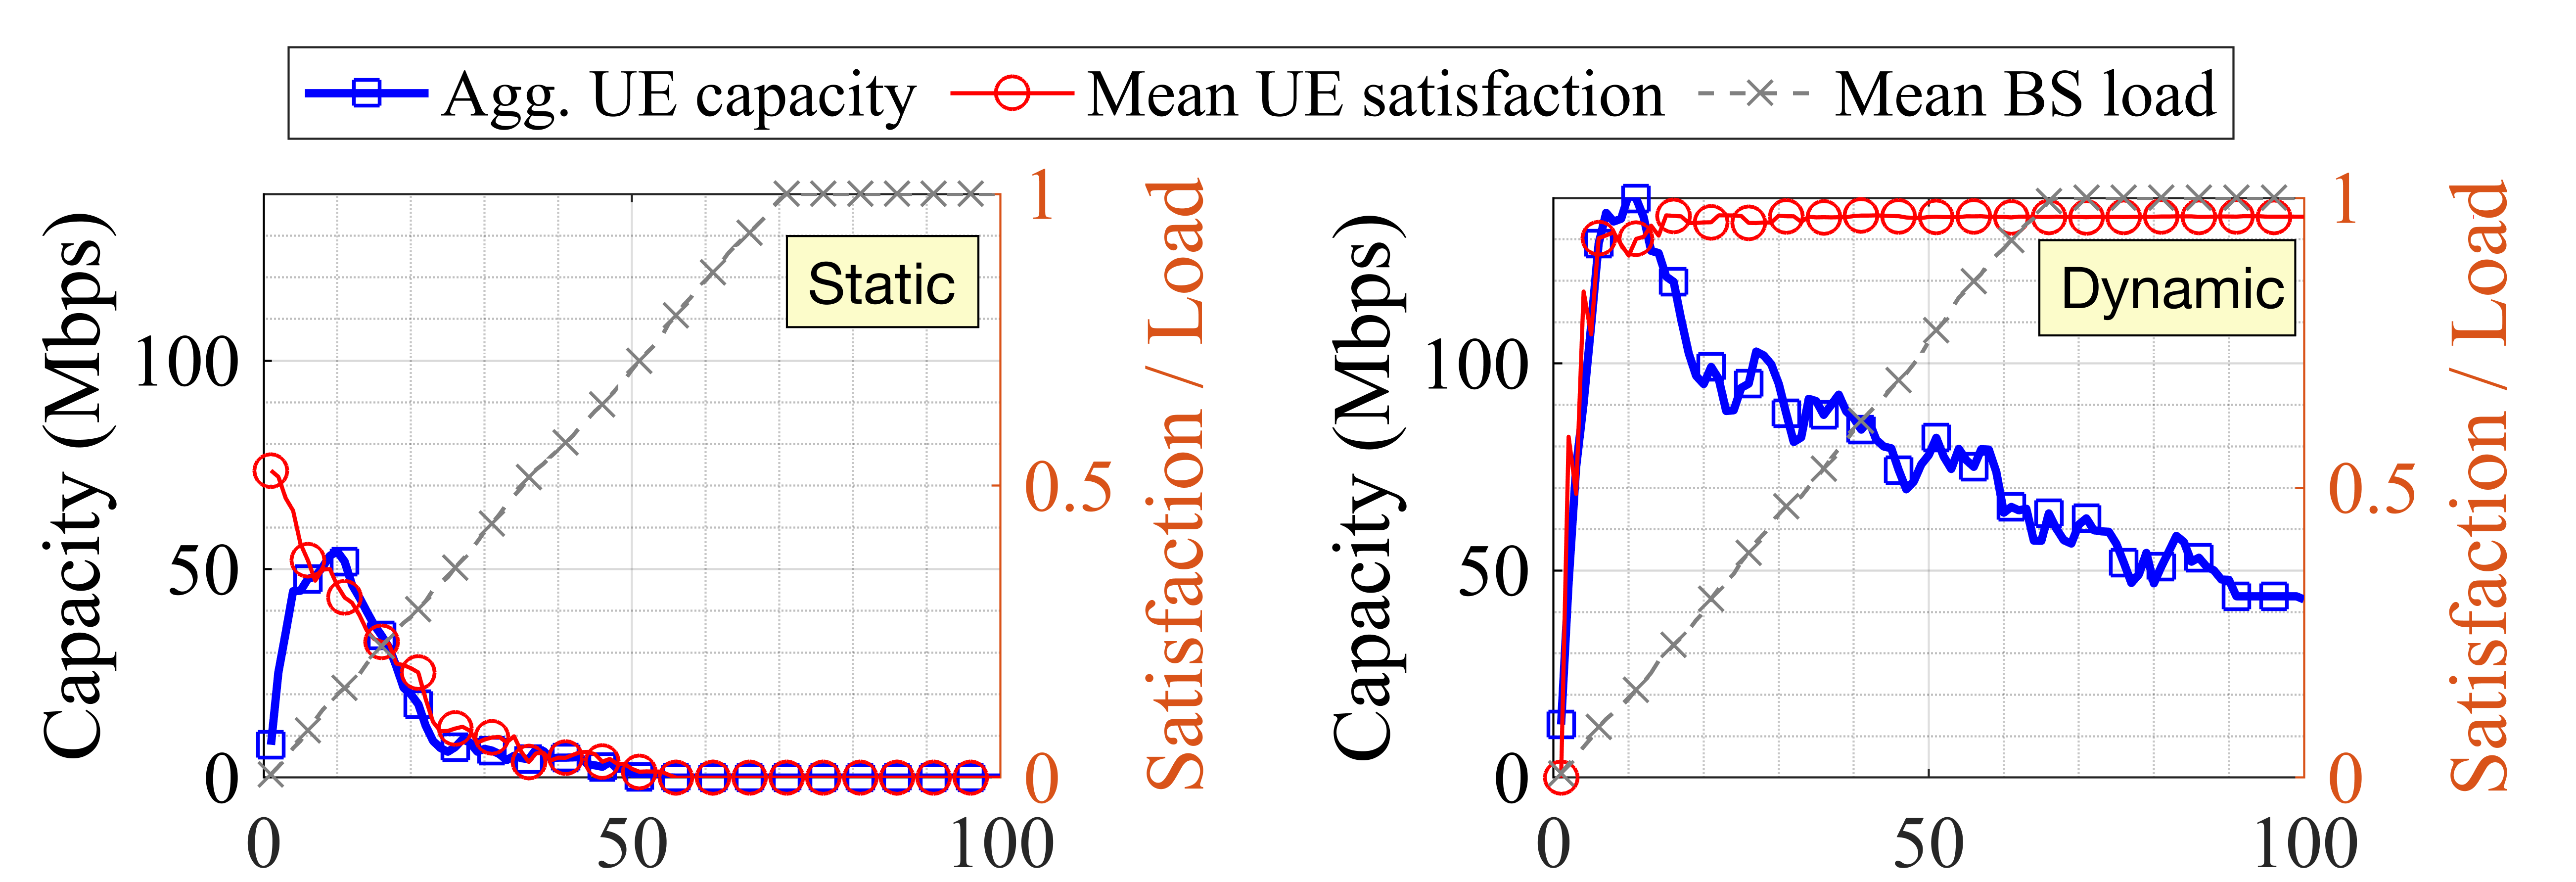
\includegraphics[width=\textwidth,keepaspectratio]{img/performance_satisfaction_1_0}\caption{\scriptsize \{1,0\} RAN ownership ratio}
		\end{figure}
		\vspace{-.8cm}
		\begin{figure}
			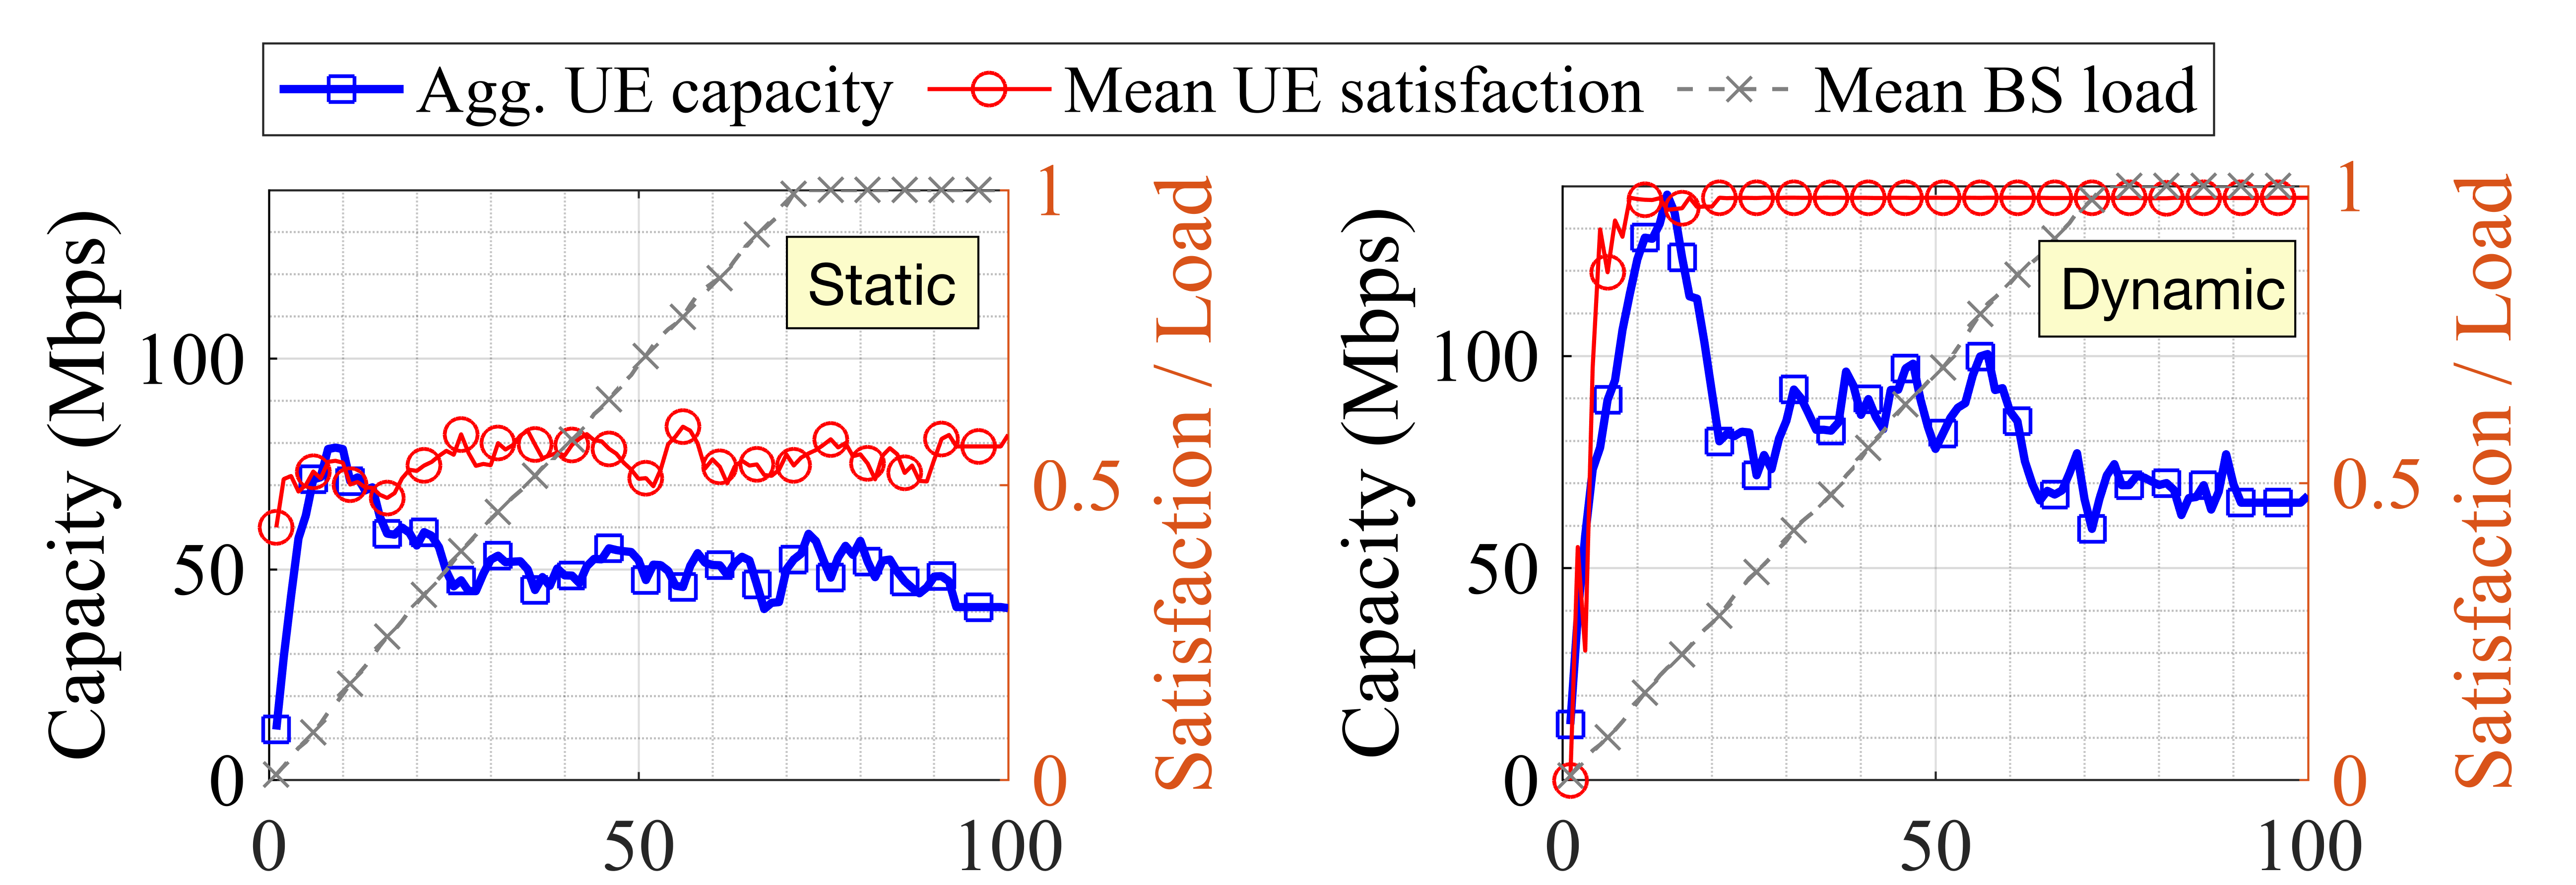
\includegraphics[width=\textwidth,keepaspectratio]{img/performance_satisfaction_05_05}\caption{\scriptsize \{0.5,0.5\} RAN ownership ratio}
		\end{figure}
	\end{column}
\end{columns}
\end{frame}

%%%%%%%%%%%%%%
%%% CONCLUSIONS
%%%%%%%%%%%%%%
\section{Conclusions}

\section{}
\begin{frame}{Conclusions}

\begin{block}{Summary}
	\begin{itemize}	
		\item Proposal to adopt BC technology for RANaaS
		\item Simulation-driven performance evaluation
	\end{itemize}
\end{block}
\pause
\begin{exampleblock}{Some conclusions}
	\begin{itemize}
		\item Fostering competitiveness is useful to reduce O\&M costs
		\item BC performance can be drastically compromised %Depending on the technology used to run a BC
		\item Links with constant  delays  (e.g.,  X2/Xn) favor BC’s operation
		\item Contention-based links (e.g., 802.11ax)  generate  high instability%, leading to re-transmissions and forks
	\end{itemize}
\end{exampleblock}
\pause
\begin{alertblock}{Ways forward}
	\begin{itemize}
		\item Architectural \& implementation aspects for BC integration
		\item Operators pricing and strategies
	\end{itemize}
\end{alertblock}

\end{frame}

%%% Questions
\section{}
\begin{frame}{Questions}
\begin{figure}
	
\includegraphics[width=\textwidth,height=0.4\textheight,keepaspectratio]{img/question_mark.png}
\end{figure}

\begin{center}
	\footnotesize
	\textbf{Francesc Wilhelmi, Ph.D.}\\
	\textcolor{blue}{fwilhelmi@cttc.cat}\\
	Centre Tecnològic de Telecomunicacions de Catalunya (CTTC)\\
	%Universitat Pompeu Fabra (Barcelona)
\end{center}

\end{frame}

% References 
\begin{frame}[allowframebreaks]{References}
\scriptsize
\bibliographystyle{amsalpha}
\bibliography{bib}
\end{frame}

\end{document}